% Created 2019-06-30 Sun 19:10
% Intended LaTeX compiler: pdflatex
\documentclass[12pt, a4paper]{article}
\usepackage[utf8]{inputenc}
\usepackage[T1]{fontenc}
\usepackage{graphicx}
\usepackage{grffile}
\usepackage{longtable}
\usepackage{wrapfig}
\usepackage{rotating}
\usepackage[normalem]{ulem}
\usepackage{amsmath}
\usepackage{textcomp}
\usepackage{amssymb}
\usepackage{capt-of}
\usepackage{hyperref}
\usepackage[style=authoryear,natbib]{biblatex}
\setlength\bibitemsep{\baselineskip}
\addbibresource{/Users/guilhermesalome/Dropbox/references.bib}
\usepackage[T1]{fontenc}
\usepackage{lmodern}
\usepackage{amsmath}
\usepackage{mathtools}
\usepackage{multirow}
\usepackage{booktabs}
\usepackage{bbm}
\usepackage{dsfont}
\usepackage[]{algorithm2e}
\newcommand\numberthis{\addtocounter{equation}{1}\tag{\theequation}}
\newcommand{\E}[1]{\mathbb{E}{\left[#1\right]}}
\newcommand{\EQ}[1]{\mathbb{E}_t^{\mathbb{Q}}{\left[#1\right]}}
\newcommand{\EP}[1]{\mathbb{E}_t^{\mathbb{P}}{\left[#1\right]}}
\newcommand{\e}[1]{\text{e}^{#1}}
\newcommand{\abs}[1]{\left\vert{#1}\right\vert}
\newcommand{\dis}{\overset{d}{\sim}}
\newcommand{\Var}[1]{\mathrm{Var}\left(#1\right)}
\newcommand{\Corr}[1]{\mathrm{Corr}\left(#1\right)}
\newcommand{\Normal}[1]{\mathcal{N}\left(0, #1\right)}
\newcommand{\Max}[1]{\text{max}\left\{#1\right\}}
\newcommand{\Set}[1]{\left\{#1\right\}}
\renewcommand{\ln}[1]{\text{ln}\left(#1\right)}
\DeclareMathOperator*{\argmin}{\arg\!\min}
\DeclareMathOperator*{\argmax}{\arg\!\max}
\DeclarePairedDelimiter\ceil{\lceil}{\rceil}
\DeclarePairedDelimiter\floor{\lfloor}{\rfloor}
\newcommand{\Poisson}[1]{\text{Poisson}\left(#1\right)}
\newcommand{\Uniform}[1]{\text{Unif}#1}
\newcommand{\Cov}[1]{\mathrm{Cov}\left(#1\right)}
\newtheorem{problem}{Problem}
\usepackage[hang,small,bf]{caption}
\usepackage[margin=1in]{geometry}
\usepackage{mathtools}
\usepackage{xcolor}
\usepackage{resizegather}
\usepackage{multirow}
\definecolor{darkgreen}{rgb}{0.1, 0.6, 0.1}
\usepackage{float}
\usepackage{listings}
\lstdefinestyle{bash}{language=bash,style=Matlab-editor,morekeywords={ssh,cd,pwd,mkdir,ls,man,rmdir,rm,nano,vim,emacs,cat,cp,mv,echo,head,tail,which}}
\usepackage{fancyhdr}
\pagestyle{fancy}
\fancypagestyle{plain}{}
\fancyhf{}
\rfoot{Page \thepage}
\usepackage{ifthen}
\rhead{\ifthenelse{\value{page}=1}{Guilherme Salom\'{e}}{Summer \the\year}}
\lhead{\ifthenelse{\value{page}=1}{Econ890-01 Matlab}{Econ890-01 Matlab}}
\usepackage[numbered,framed]{matlab-prettifier}
\usepackage{listings}
\date{}
\title{Speeding Code Execution with the Econ Cluster}
\hypersetup{
 pdfauthor={Guilherme Salomé},
 pdftitle={Speeding Code Execution with the Econ Cluster},
 pdfkeywords={},
 pdfsubject={},
 pdfcreator={Emacs 26.1 (Org mode 9.2.1)},
 pdflang={English}}
\begin{document}

\maketitle
For most tasks, it is often enough to execute code on your own computer.
And for most tasks, using a single core of a processor is also enough.
However, there are compute intensive tasks that can greatly benefit from a computer with several cores and access to a relevant amount of memory.
For these tasks, your own computer might not suffice.
Fortunately, the Economics Department at Duke has its own cluster of computers that Master's and PhD students can use.
\section{Requesting Access to the Cluster}
\label{sec:org5ee5c2a}
To access the cluster, you will need a username and password.
The username for the Econ Cluster is the same as your University NetID username, but the password is different.
If you do not have a password yet, or do not remember it (if you are a PhD student you were probably assigned a password during your 1st year at Duke), you can request a password by emailing \href{mailto:help@econ.duke.edu}{help@econ.duke.edu}.
\section{Connecting to the Cluster}
\label{sec:org489e288}
You can think of the Econ Cluster as a collection of several computers, which are managed by some centralized software.
One of these computers is responsible for handling log in, and is known as the front-end node (or the login node).
This node is also responsible for receiving and scheduling tasks on the other computers in the cluster.

To log in the Econ Cluster we will use the \href{https://en.wikipedia.org/wiki/Secure\_Shell}{SSH} protocol.
This protocol was designed to allow two computers to securely communicate over an insecure network.
If you are using a Mac or Linux-based operating system (like Ubuntu), then you already have what is required to use SSH.
If you are on Windows, then you will need to install an SSH client, like \href{https://www.chiark.greenend.org.uk/\~sgtatham/putty/}{PuTTY} or any of the \href{https://www.puttygen.com/best-putty-alternatives-ssh-clients}{alternatives} (they are all similar and straightforward).
\subsection{Mac, Ubuntu or Linux}
\label{sec:org07888b6}
Open the \href{https://support.apple.com/guide/terminal/welcome/mac}{Terminal} program. You should see a window similar to the one depicted in Figure \ref{fig:org0e48c20}.

\begin{figure}[H]
\centering
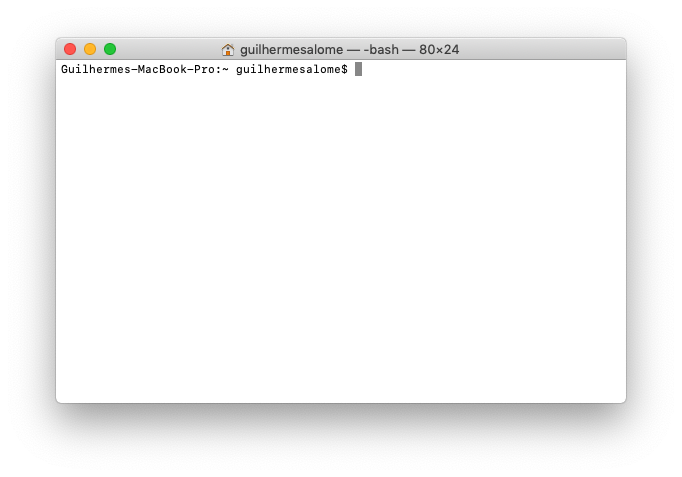
\includegraphics[width=8cm]{/Users/guilhermesalome/Teaching/Duke/Econ890 Matlab - 2019/supporting/matlab_terminal_mac.png}
\caption{\label{fig:org0e48c20}
Terminal on a Mac.}
\end{figure}

You can type commands after the dollar sign, and the terminal will interpret the commands and execute them (REPL).
We will discuss how to use the terminal in the next section.

To log in the Econ Cluster, we will the the \texttt{ssh} command.
The \texttt{ssh} command uses the syntax:
\lstset{language=bash,label= ,caption= ,captionpos=b,firstnumber=1,numbers=left,style=bash}
\begin{lstlisting}
ssh username@hostname
\end{lstlisting}
Where \texttt{username} is the username you will use to log in, and \texttt{hostname} is the address of the computer host that you will connect to.
If you are currently inside the Duke network, then the \texttt{hostname} is \texttt{login.econ.duke.edu}.
In my case, I would execute:
\lstset{language=bash,label= ,caption= ,captionpos=b,firstnumber=1,numbers=left,style=bash}
\begin{lstlisting}
ssh gfs8@login.econ.duke.edu
\end{lstlisting}
Then, I am asked for my password to finish logging in (see Figure \ref{fig:orgfbdea8d}).

\begin{figure}[H]
\centering
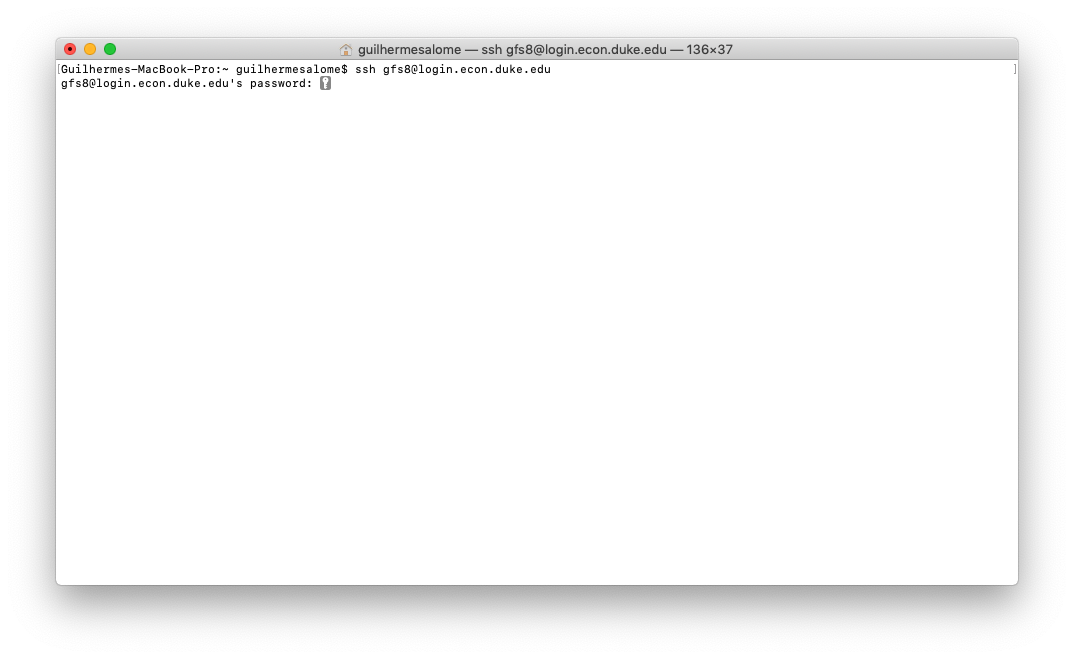
\includegraphics[width=8cm]{/Users/guilhermesalome/Teaching/Duke/Econ890 Matlab - 2019/supporting/matlab_ssh_password.png}
\caption{\label{fig:orgfbdea8d}
SSH Asking for Password.}
\end{figure}

After typing your password, you should be greeted with a welcome message and are now connected to the cluster (see Figure \ref{fig:orgd27beb3}).
You are connected to a \href{https://en.wikipedia.org/wiki/Bash\_(Unix\_shell)}{bash} terminal, which can take commands and will execute them.
We will discuss these commands in the next section.

\begin{figure}[H]
\centering
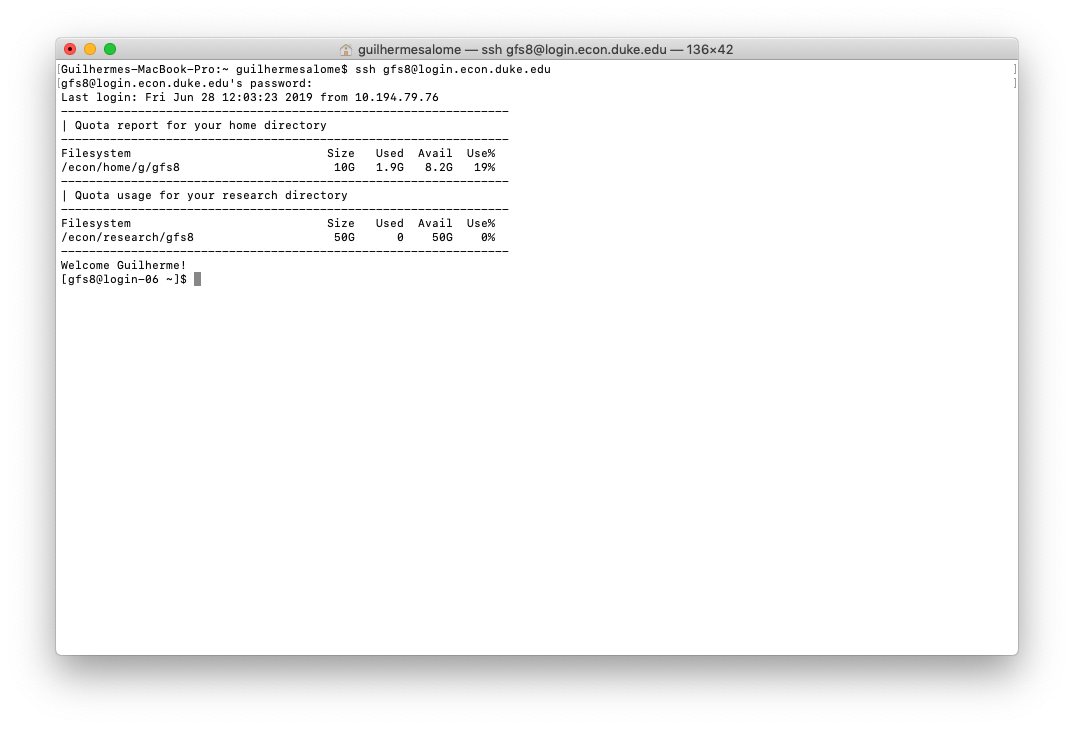
\includegraphics[width=8cm]{/Users/guilhermesalome/Teaching/Duke/Econ890 Matlab - 2019/supporting/matlab_ssh_logged_in.png}
\caption{\label{fig:orgd27beb3}
SSH Welcome Message.}
\end{figure}

If you are outside the Duke network, then you first the need to \texttt{ssh} into the Duke network, and then \texttt{ssh} again into the Econ Cluster.
To \texttt{ssh} into the Duke network, you should use \texttt{login.oit.duke.edu} as the \texttt{hostname}, but now the username and password are the same you use for logging into Duke websites (like Dukehub).
After that, you can execute \texttt{ssh} again to log in the Econ Cluster (see Figure \ref{fig:orge73a9c7}).

\begin{figure}[H]
\centering
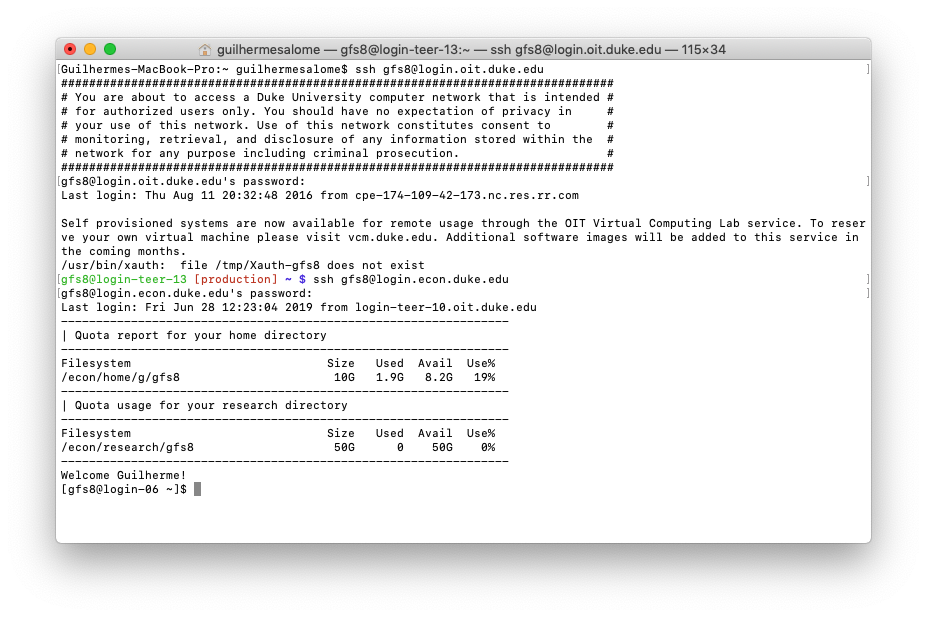
\includegraphics[width=8cm]{/Users/guilhermesalome/Teaching/Duke/Econ890 Matlab - 2019/supporting/matlab_ssh_from_outside.png}
\caption{\label{fig:orge73a9c7}
SSH From Outside Duke Network.}
\end{figure}
\subsection{Windows}
\label{sec:orga69e4ce}
To connect to the cluster when working in the Windows operating system, you will need to install an SSH client.
I recommend installing \href{https://www.chiark.greenend.org.uk/\~sgtatham/putty/}{PuTTY} due to its simplicity and convenience (it is also free).
After installing the software, you will use \texttt{ssh} but with a graphical user interface.

Open PuTTY and type \texttt{login.econ.duke.edu} on the \texttt{Host Name} window (see Figure \ref{fig:org2daae6c}).
You can now click \texttt{Open} to connect to the cluster.
You will be prompted for your username and your password.

\begin{figure}[H]
\centering
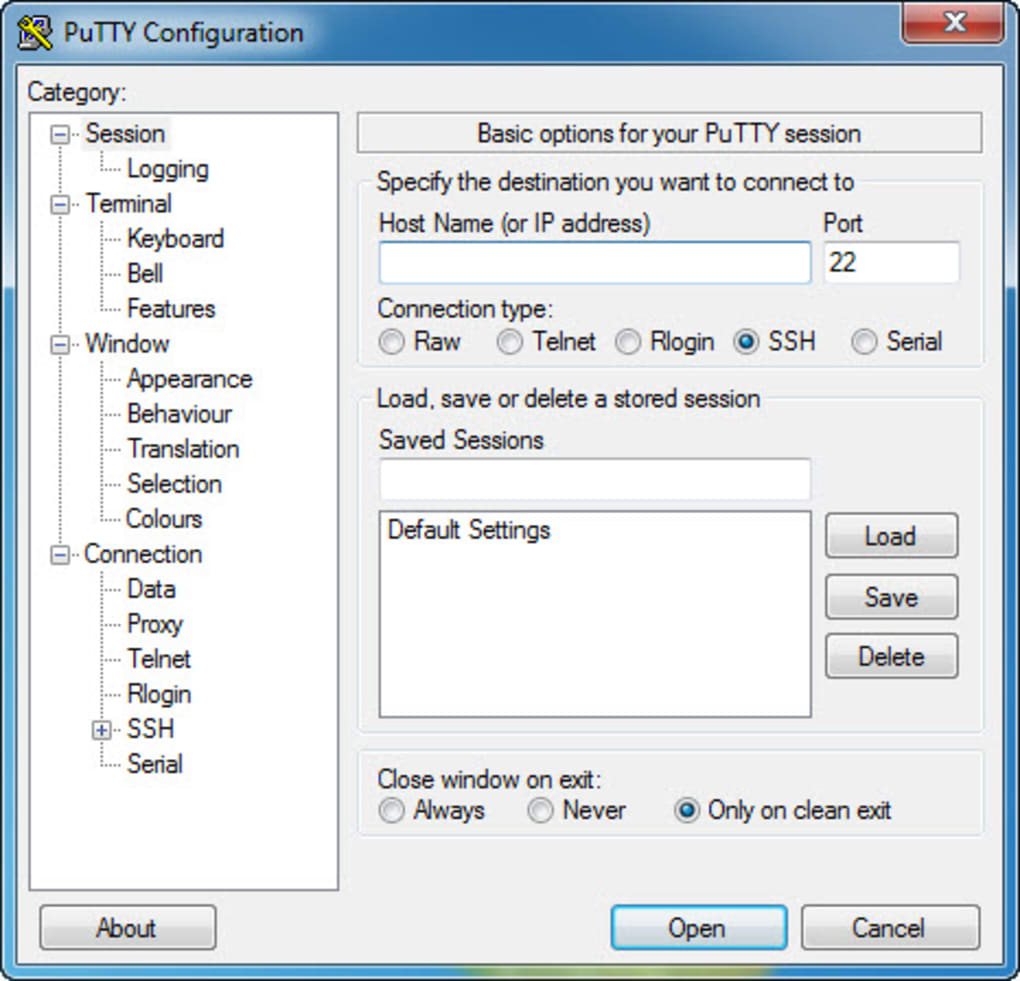
\includegraphics[width=8cm]{/Users/guilhermesalome/Teaching/Duke/Econ890 Matlab - 2019/supporting/matlab_putty.jpg}
\caption{\label{fig:org2daae6c}
PuTTY SSH Client.}
\end{figure}

After typing your password, you should be greeted with a welcome message and are now connected to the cluster.
You are connected to a \href{https://en.wikipedia.org/wiki/Bash\_(Unix\_shell)}{bash} terminal, which can take commands and will execute them.
We will discuss these commands in the next section.

\section{Using a Bash Terminal}
\label{sec:orgd81750d}
Now that we are connected to the cluster, we can discuss how to use the terminal.
The terminal window you see is a bash shell.
A shell is just a user interface to the underlying operating system, and bash refers to the type of interface.

We can interact with the shell either by typing commands and executing them line by line, or by creating script files.
We will cover some basic commands of the bash shell.
\subsection{Working Directory}
\label{sec:org5e5265b}
The command \texttt{pwd} prints the current working directory:
\lstset{language=bash,label= ,caption= ,captionpos=b,firstnumber=1,numbers=left,style=bash}
\begin{lstlisting}
pwd
\end{lstlisting}
You can change the working directory with the \texttt{cd} command:
\lstset{language=bash,label= ,caption= ,captionpos=b,firstnumber=1,numbers=left,style=bash}
\begin{lstlisting}
# syntax: cd folder
cd /econ
pwd
cd /econ/home
pwd
cd /econ/home/g/gfs8
pwd
cd ..				# .. refers to the parent folder
pwd
\end{lstlisting}
While \texttt{..} represents the parent folder, there is a shortcut for your home folder as well:
\lstset{language=bash,label= ,caption= ,captionpos=b,firstnumber=1,numbers=left,style=bash}
\begin{lstlisting}
cd ~
# ~ represents the home folder
# alternatively
cd $HOME
\end{lstlisting}
\subsection{Creating Folders}
\label{sec:orgc12b9a8}
You have permission to change things around only in your home folder.
In my case, my home folder is the folder \texttt{/econ/home/g/gfs8}.
We can create a new folder with the command \texttt{mkdir}:
\lstset{language=bash,label= ,caption= ,captionpos=b,firstnumber=1,numbers=left,style=bash}
\begin{lstlisting}
# syntax: mkdir folder_name
mkdir Matlab
mkdir Test
# create multiple folders
mkdir A B C
\end{lstlisting}
\subsection{Listing Files and Folders}
\label{sec:org4183341}
We can list all files and folders inside a folder with the command \texttt{ls}.
\lstset{language=bash,label= ,caption= ,captionpos=b,firstnumber=1,numbers=left,style=bash}
\begin{lstlisting}
# syntax: ls
ls
# display one file or folder per line
ls -1
\end{lstlisting}
You can get a full list of the options a command accepts by reading the manual page of the command.
You can access the manual page of a command using \texttt{man}:
\lstset{language=bash,label= ,caption= ,captionpos=b,firstnumber=1,numbers=left,style=bash}
\begin{lstlisting}
# syntax: man command_name
man ls
\end{lstlisting}
\subsection{Deleting Files and Folders}
\label{sec:org0c7a8b5}
We can delete an empty folder with the command \texttt{rmdir}.
\lstset{language=bash,label= ,caption= ,captionpos=b,firstnumber=1,numbers=left,style=bash}
\begin{lstlisting}
# syntax: rmdir folder_name
rmdir Test
# remove multiple folders
rmdir A B C
\end{lstlisting}
To remove a non-empty folder we need to use the more versatile command \texttt{rm} with the option \texttt{-r}:
\lstset{language=bash,label= ,caption= ,captionpos=b,firstnumber=1,numbers=left,style=bash}
\begin{lstlisting}
# create a non-empty folder
mkdir Test Test/A Test/B
# check it is non-empty
ls -1 Test
# equivalent to
cd Test
ls -1
cd ..
# try to remove with rmdir
rmdir Test			# error
# use rm -r
rm -r Test			# works
\end{lstlisting}
The command \texttt{rm} can also be used to remove files.
\subsection{Creating Files}
\label{sec:org6fc6038}
We can create empty files with the \texttt{touch} command:
\lstset{language=bash,label= ,caption= ,captionpos=b,firstnumber=1,numbers=left,style=bash}
\begin{lstlisting}
# syntax: touch file_name
touch test.txt
# create multiple files
touch a.csv b.jpg
# remove files
rm test.txt
# remove multiple files
rm a.csv b.jpg
\end{lstlisting}
We can also create and edit files.
To edit a file we need an editor.
Some of the editors available inside the bash terminal are: \href{https://www.nano-editor.org}{nano}, \href{https://www.vim.org}{vim} and \href{https://www.gnu.org/software/emacs/}{emacs}.
You can create or edit a file with these editors by typing the name of the editor followed by the name of the file.
The editor \texttt{nano} is the most straightforward to use, however, the editors \texttt{vim} and \texttt{emacs} are extremely powerful and might be worth to learn if you often use your computer to type text into files.
\lstset{language=bash,label= ,caption= ,captionpos=b,firstnumber=1,numbers=left,style=bash}
\begin{lstlisting}
# create a new file with nano
nano data.csv
# nano will now open with an empty file
# type in:
# 1,21,0
# 2,28,25000
# 3,35,70000
# then use Ctrl-O to save the file, and then Ctrl-X to exit nano
# create another file
nano description.txt
# type in:
# id,age,income
\end{lstlisting}
\subsection{Inspecting Files}
\label{sec:orgf2226e4}
You can quickly inspect the contents of a file with the \texttt{cat} command.
\lstset{language=bash,label= ,caption= ,captionpos=b,firstnumber=1,numbers=left,style=bash}
\begin{lstlisting}
# check name of files
ls -1
# see contents of data.csv
cat data.csv
# see contents of description.txt and data.csv
cat description.txt data.csv
\end{lstlisting}
If the file is too big and you do not want to display its entirety on the screen, you can use the \texttt{head} and \texttt{tail} commands.
The \texttt{head} command displays the first few lines of a file, while the \texttt{tail} command displays the last lines of a file.
\lstset{language=bash,label= ,caption= ,captionpos=b,firstnumber=1,numbers=left,style=bash}
\begin{lstlisting}
# see first lines of the file
head data.csv
# see only first two lines of the file
head -n 2 data.csv
# see only the first line of the file
head -n 1 data.csv
# see last lines of the file
tail data.csv
# see only very last line of the file
tail -n 1 data.csv
# display first line of multiple files
head -n 1 description.txt data.csv
\end{lstlisting}
\subsection{Copying and Moving Files}
\label{sec:org239e73b}
To copy files use the \texttt{cp} command.
\lstset{language=bash,label= ,caption= ,captionpos=b,firstnumber=1,numbers=left,style=bash}
\begin{lstlisting}
# syntax: cp source_file target_file
# create a copy of data.csv
cp data.csv data_copy.csv
# create a copy of the data inside a data folder
mkdir Data
cp data.csv Data/
ls Data
\end{lstlisting}
Files can be moved with the \texttt{mv} command.
\lstset{language=bash,label= ,caption= ,captionpos=b,firstnumber=1,numbers=left,style=bash}
\begin{lstlisting}
# remove the copy of data.csv from the Data folder
rm Data/data.csv
ls Data
# move the original data file to the Data folder
mv data.csv Data/
# check the file changed folder
ls
ls Data
\end{lstlisting}
\section{Bash scripts}
\label{sec:orgcdaf319}
A bash script is just like a Matlab script: it is a text file containing commands that should be executed line by line.
We can create a bash script by creating a file with the extension \texttt{.sh}.
Let's use the command \texttt{echo} to print strings to the terminal window and save them in a script file.

\lstset{language=bash,label= ,caption= ,captionpos=b,firstnumber=1,numbers=left,style=bash}
\begin{lstlisting}
# syntax: echo string
echo "Hello there!"
echo "How are you?"
\end{lstlisting}
Save it in a file (\texttt{nano greetings.sh}):

\lstset{language=bash,label= ,caption= ,captionpos=b,firstnumber=1,numbers=left,style=bash}
\begin{lstlisting}
# greetings.sh
echo "Hello there!"
echo "This is a bash terminal."
echo "Welcome."
head data.csv
\end{lstlisting}

We can execute this file with the command \texttt{source}.
The \texttt{source} command takes a script file and executes it line by line in the current shell.
\lstset{language=bash,label= ,caption= ,captionpos=b,firstnumber=1,numbers=left,style=bash}
\begin{lstlisting}
# syntax: source script_name
source greetings.sh
\end{lstlisting}
And you should see the three messages displayed in the shell.

We can use a shell script to execute several programs, including programs in other languages.
To do so, the shell must be able to find other programs.
For example, when we typed \texttt{nano} before, the shell searched for the program \texttt{nano} and then executed it with the parameters we passed it.
We can check whether the terminal can find a program with the command \texttt{which}.
\lstset{language=bash,label= ,caption= ,captionpos=b,firstnumber=1,numbers=left,style=bash}
\begin{lstlisting}
# syntax: which program_name
# if the program can be found, then the shell
# displays the path to the program binaries
which nano
which emacs
# if the program cannot be found, then nothing is displayed
which foo123
\end{lstlisting}
If the program cannot be found, then it could either not be available in the machine, or it could be outside of the path of the terminal.
The path is a list of folders where the terminal searches for programs.
If the program cannot be found in those folders, then the terminal does not return anything.
However, if you know in which folder the program lives, then you can specify the full path to it.
Alternatively, you can add its folder to the search path (this is left for another time, as it introduces some complications).
For example, in my machine \texttt{matlab} is not in the search path, but it can be found by specifying the full path:
\lstset{language=bash,label= ,caption= ,captionpos=b,firstnumber=1,numbers=left,style=bash}
\begin{lstlisting}
# on local machine
which matlab
# returns nothing
# but we can specify the full path
which /Applications/MATLAB_R2019a.app/bin/matlab
\end{lstlisting}

On the cluster, however, \texttt{matlab} should be in the search path:
\lstset{language=bash,label= ,caption= ,captionpos=b,firstnumber=1,numbers=left,style=bash}
\begin{lstlisting}
ssh gfs8@login.econ.duke.edu
which matlab
# returns /usr/local/bin/matlab
\end{lstlisting}

Let's create a Matlab script that will perform some computation and save the results.
\lstset{language=matlab,label= ,caption= ,captionpos=b,firstnumber=1,numbers=left,style=Matlab-editor}
\begin{lstlisting}
% matlab_computation.m
% Do some computation
x = rand(200, 1);
y = rand(200, 1);
res = x.*y.^2 + 1;
% Save results
save('results.mat', 'res');
\end{lstlisting}

We can now write a bash script that will interact with the operating system and then execute the Matlab script.
To execute the Matlab script we would call \texttt{matlab test.m}.
However, \texttt{matlab} also takes some options that can speed up its execution.
We can pass a script to be executed with \texttt{matlab} by using the option \texttt{-batch} and specifying the script name, without the extension \texttt{.m}.
The complete set of options \texttt{matlab} takes is described in \href{https://www.mathworks.com/help/matlab/ref/matlablinux.html?s\_tid}{this reference page}.
\lstset{language=bash,label= ,caption= ,captionpos=b,firstnumber=1,numbers=left,style=bash}
\begin{lstlisting}
# matlab_from_bash.sh
echo "Executes the Matlab script: matlab_computation.m"
# execute Matlab script
matlab -batch "matlab_computation"
\end{lstlisting}
We can now execute this script with \texttt{source matlab\_from\_bash.sh}, and the script will be executed.
Notice that at the end of the script, Matlab saves the results in the file \texttt{results.mat}, which later we can import into our computer to analyze.
\section{Slurm: Scheduling Tasks}
\label{sec:org885da08}
Bash scripts are important because they are how we can interact with the Econ Cluster.
Remember, the Cluster is simply a collection of computers being managed by some software.
The software that manages the Econ Cluster is the \href{https://en.wikipedia.org/wiki/Slurm\_Workload\_Manager}{Slurm Workload Manager}.

In the previous section, we logged in the log-in node of the cluster.
At that node, we can interact with the cluster via the terminal, and even execute some Matlab code via a \texttt{bash} script.
However, Slurm will not allow us to execute a lot of code, or code that takes too long to run.
Instead, Slurm allows us to submit tasks for it to run.
That is, we can give Slurm a \texttt{bash} script, and it will allocate the script to some computer in the cluster, run it, and save the results in your home folder.
In doing so, Slurm allows all users of the Cluster access to powerful computers, but there may be a queue.
\subsection{Shebang}
\label{sec:orga6d4257}
The script \texttt{matlab\_from\_bash.sh} is almost ready to be submitted for execution with Slurm.
It is only missing a \href{https://en.wikipedia.org/wiki/Shebang\_(Unix)}{shebang} line.
The shebang is the very first line of a text file used as a script, which specifies the interpreter that should be used when executing the file.
While we could execute our script with \texttt{source}, by adding a shebang to the file, we can execute it as an executable file.
Create the following test script:
\lstset{language=bash,label= ,caption= ,captionpos=b,firstnumber=1,numbers=left,style=bash}
\begin{lstlisting}
#!/bin/bash
# test_shebang.sh
echo "Hello!"
\end{lstlisting}
We can still execute it with \texttt{source}:
\lstset{language=bash,label= ,caption= ,captionpos=b,firstnumber=1,numbers=left,style=bash}
\begin{lstlisting}
source test_shebang.sh
\end{lstlisting}
But now, we can execute it as an executable file:
\lstset{language=bash,label= ,caption= ,captionpos=b,firstnumber=1,numbers=left,style=bash}
\begin{lstlisting}
# make the file executable
chmod +x test_shebang.sh
# execute it
./test_shebang.sh
\end{lstlisting}
The first line of the script tells the terminal that it should use \texttt{bash} to interpret its contents.
Slurm needs this shebang to correctly submit the script.
\subsection{Submitting to the Cluster}
\label{sec:orgb60eea2}
Modify the \texttt{matlab\_from\_bash.sh} so that its first line is \texttt{\#!/bin/bash}.
Delete the \texttt{results.mat} file from the folder.

We can submit the \texttt{matlab\_from\_bash.sh} script to Slurm with the command \texttt{sbatch}.
\lstset{language=bash,label= ,caption= ,captionpos=b,firstnumber=1,numbers=left,style=bash}
\begin{lstlisting}
# submit script to Slurm
sbatch matlab_from_bash.sh
\end{lstlisting}
If there is no immediate issue with the script, Slurm will schedule the script for execution in one of the computers (nodes) of the cluster.
The scheduled script is called a job.
Slurm will print the job number on the screen.
\subsection{The Queue}
\label{sec:org700b69f}
After submitting a script for execution, you should have its job number.
You can use this number to check what is the state of the job.
We can use the command \texttt{squeue} to see all jobs currently scheduled and being executed.
See Figure \ref{fig:org0cb56e0} for the output of \texttt{squeue}

\begin{figure}[H]
\centering
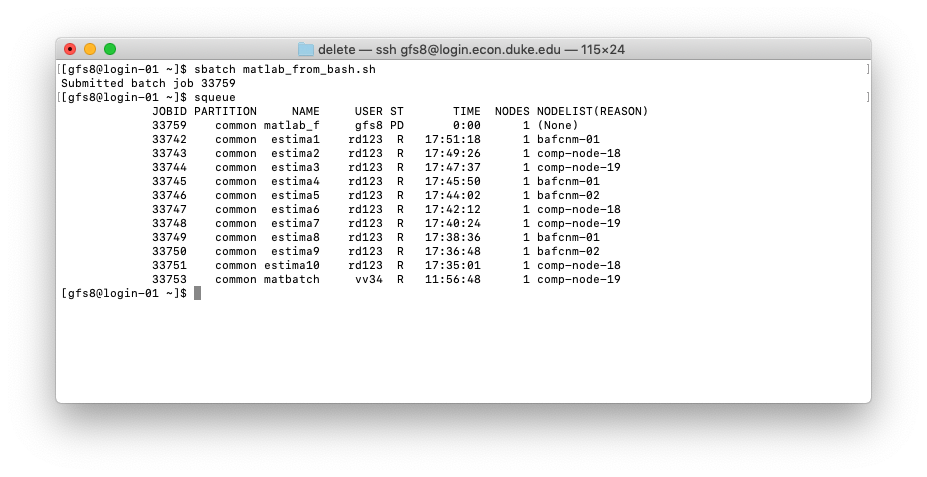
\includegraphics[width=8cm]{/Users/guilhermesalome/Teaching/Duke/Econ890 Matlab - 2019/supporting/matlab_squeue.png}
\caption{\label{fig:org0cb56e0}
Slurm queue after submitting a job.}
\end{figure}

The job we just submitted has the number \texttt{33759}.
You can see in the second line after the command \texttt{squeue} that the job has been scheduled.
The \texttt{NAME} shows the name of the script submitted, \texttt{USER} shows the user who submitted the job (net id), \texttt{ST} shows the state of the job (PD stands for pending, while R stands for running).
The \texttt{TIME} shows for how long the job has been running.
In the case of our job it has not started yet, so \texttt{TIME} is \texttt{0:00}.
Notice that some other users have jobs running for more than 17 hours!
The \texttt{NODELIST} describes the reason why the job is in the queue.
In the case of the job we submitted, \texttt{(None)} means the job will be executed next.
Usually, if there are not enough resources available to execute your script, you will see a \texttt{(Resources)}, which indicates Slurm is waiting for other scripts to finish before executing yours.
When the script is being executed, \texttt{NODELIST} will show the node (computer) where the script is running.

If we have multiple jobs running, then we can check the status of the jobs submitted only by us (not by everyone).
We can do so with the option \texttt{-u username}, which displays \texttt{squeue} but only for the specified username.
\lstset{language=bash,label= ,caption= ,captionpos=b,firstnumber=1,numbers=left,style=bash}
\begin{lstlisting}
squeue -u gfs8
\end{lstlisting}

See Figure \ref{fig:org7e64344} for an example.
\begin{figure}[H]
\centering
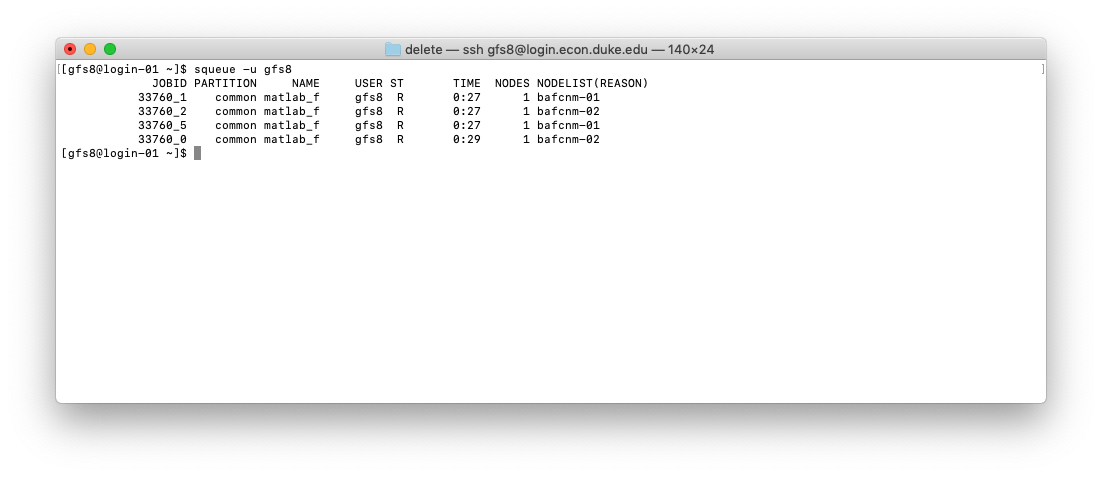
\includegraphics[width=8cm]{/Users/guilhermesalome/Teaching/Duke/Econ890 Matlab - 2019/supporting/matlab_squeue_username.png}
\caption{\label{fig:org7e64344}
View of Slurm queue for a specified user.}
\end{figure}

In this case I submitted several jobs.
The queue shows they are all running, some are running on different nodes, and they have been running for a few seconds already.
If you run \texttt{squeue -u gfs8} again, then you might see fewer jobs.
This is because when a job is completed, it does not show up in the queue anymore.
\subsection{Details on a Job}
\label{sec:org425be05}
We can use the \texttt{sacct} to get information on running and completed jobs we have submitted to Slurm.
Running \texttt{sacct} will display details for all jobs submitted by you on a certain period of time.
If you have the job number, then you can use pass it with the option \texttt{-j} to get details about that specific job (see Figure \ref{fig:org1a2eb85}):
\lstset{language=bash,label= ,caption= ,captionpos=b,firstnumber=1,numbers=left,style=bash}
\begin{lstlisting}
sacct -j 33759
\end{lstlisting}

\begin{figure}[H]
\centering
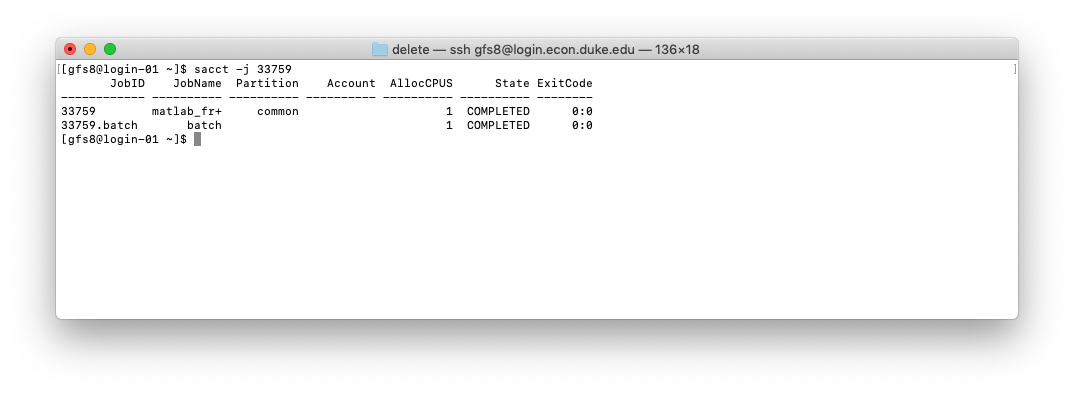
\includegraphics[width=8cm]{/Users/guilhermesalome/Teaching/Duke/Econ890 Matlab - 2019/supporting/matlab_sacct_job.png}
\caption{\label{fig:org1a2eb85}
View details of a submitted job.}
\end{figure}

If you want even more information about a specific job, then you can use the command \texttt{sacct\_ec}:
\lstset{language=bash,label= ,caption= ,captionpos=b,firstnumber=1,numbers=left,style=bash}
\begin{lstlisting}
sacct_ec -j 33759
\end{lstlisting}

Figure \ref{fig:orgb271ff2} displays the output of \texttt{sacct\_ec}.
Notice it shows the node where the script was executed, and even the start and end time of the script.

\begin{figure}[H]
\centering
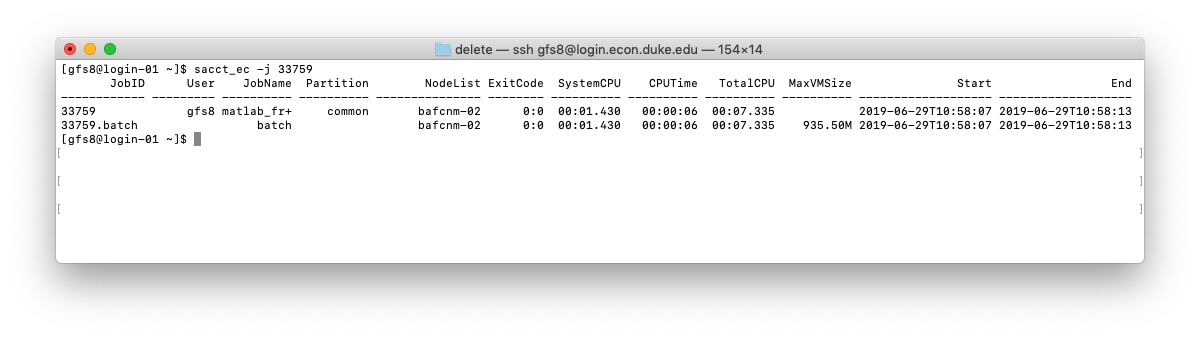
\includegraphics[width=8cm]{/Users/guilhermesalome/Teaching/Duke/Econ890 Matlab - 2019/supporting/matlab_sacct_ec.png}
\caption{\label{fig:orgb271ff2}
View even more details of a submitted job.}
\end{figure}

These commands are useful when you submit jobs that might take a long time to execute, or when debugging scripts that are failing to execute.
\subsection{Canceling a Job}
\label{sec:org2d469a7}
You can cancel a job using the \texttt{scancel} command.
For example, if the job number is 33759, then \texttt{scancel 33759} will cancel the job.
You can only cancel jobs you started yourself.
If your script is taking longer than expected to complete, then you might have some bug in your code that is causing it to hang.
In this case, canceling the job might be required.
\subsection{Outputs of the Job}
\label{sec:orgdf2bc2e}
When a job is submitted and starts running, a file with the name \texttt{slurm-XXXXX.out} is created.
The \texttt{XXXXX} represents the number of the corresponding job.
This file contains whatever your script prints to the screen.
For example, when we executed the \texttt{matlab\_from\_bash.sh} script, it printed a couple of lines on the terminal.
If we submit this script to Slurm, then the lines that would be printed on the terminal are saved on the \texttt{slurm-XXXXX.out} file.

The \texttt{.out} file can be used as a log of what is happening in your script.
You can use it to debug your program, since debugging in the cluster is not as straightforward as debugging in your local machine (you cannot stop the execution of the code and inspect variables, for example).

The Matlab script we submitted also created a file containing the results. This file is also saved in our home folder.
When we submit a job with Slurm, our home folder is directly accessible by the job, and behaves as a local drive.

\section{Slurm: Partitions and Nodes}
\label{sec:org423e3eb}
Slurm organizes the cluster in \texttt{partitions}, where each \texttt{partition} is a set of \texttt{compute nodes} (computers used to run code).
We can get an overview of the partitions available in the Econ Cluster with the \texttt{sinfo} command.
Figure \ref{fig:org962275b} displays the output of \texttt{sinfo}.

\begin{figure}[H]
\centering
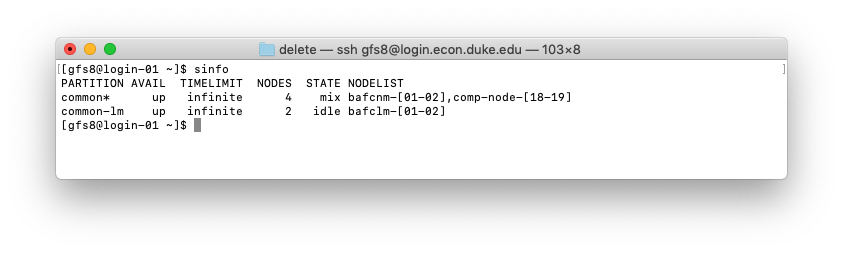
\includegraphics[width=8cm]{/Users/guilhermesalome/Teaching/Duke/Econ890 Matlab - 2019/supporting/matlab_sinfo.png}
\caption{\label{fig:org962275b}
Overview of cluster partitions.}
\end{figure}

Notice there are two partitions, \texttt{common*} and \texttt{common-lm}.
Different partitions might have different purposes.
For example, there could be a partition for debugging code, and another for actually submitting tasks.
In this case, the two partitions are for computing.
The default partition is marked with an asterisk.
That is, the partition \texttt{common} is where jobs are submitted to by default.

There are four compute nodes in the default partition. Some of them are in use, other are idle, leading to the \texttt{mix} state.
In the \texttt{common-lm} partition there are two nodes, which are idle.
The \texttt{NODELIST} column gives the names of the nodes.
The nodes in the \texttt{common} partition are \texttt{bafcnm-01}, \texttt{bafcnm-02}, \texttt{comp-node-18} and \texttt{comp-node-19}.
The nodes in the \texttt{common-lm} partition are \texttt{bafclnm-01} and \texttt{bafcnm-02}.

Notice that the column \texttt{TIMELIMIT} says \texttt{infinite}.
This is the time limit to which jobs are subject.
In this case, there is no time limit.

We can display information organized by node instead of partition with the option \texttt{-N}. We can also use the option \texttt{-l} to display extra information.
\lstset{language=bash,label= ,caption= ,captionpos=b,firstnumber=1,numbers=left,style=bash}
\begin{lstlisting}
sinfo -N -l
\end{lstlisting}

Figure \ref{fig:org9834cf6} displays the output of \texttt{sinfo -N -l}.
\begin{figure}[H]
\centering
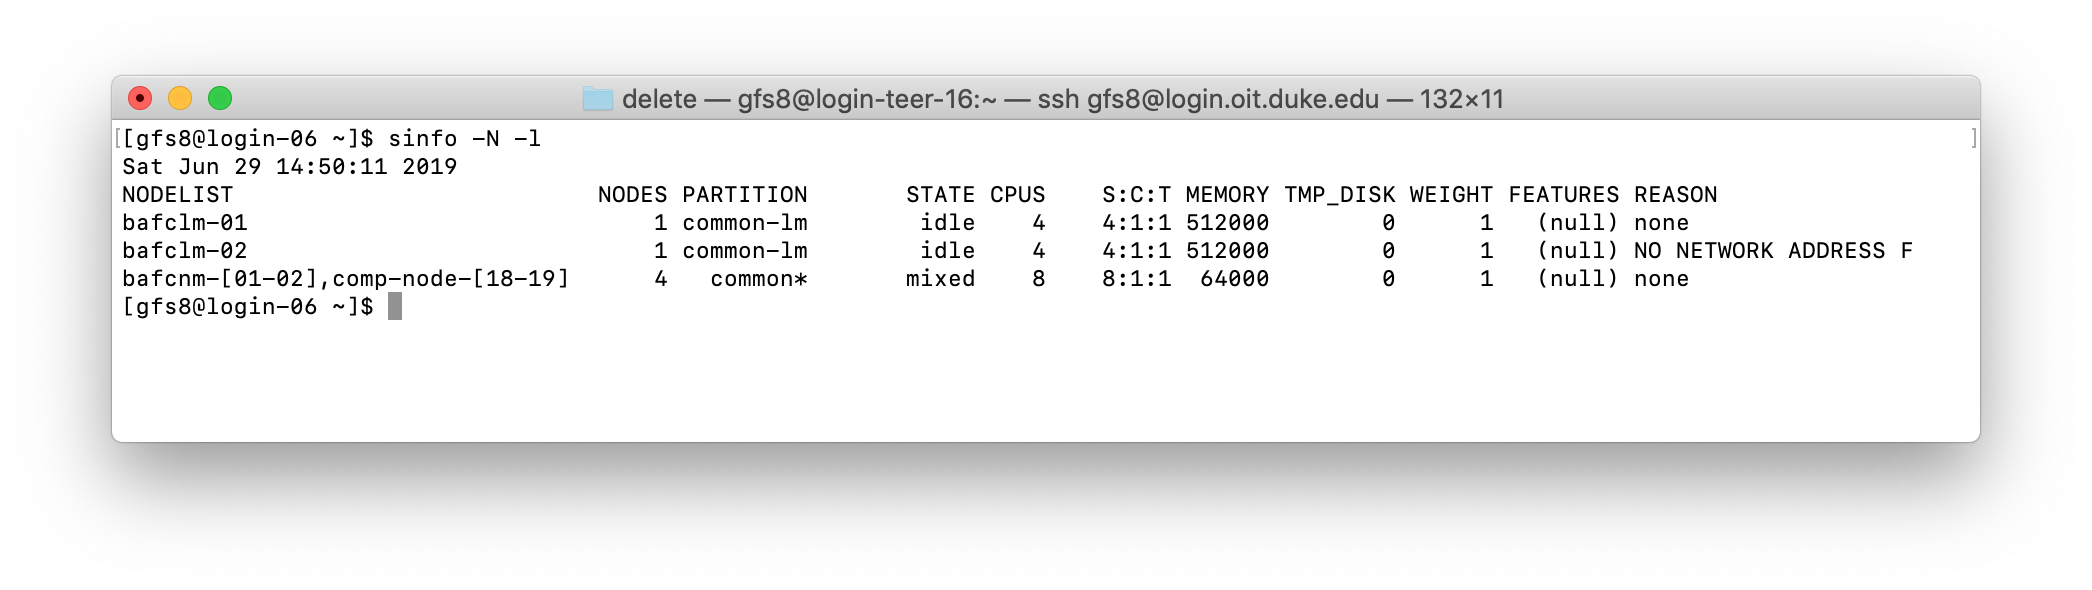
\includegraphics[width=8cm]{/Users/guilhermesalome/Teaching/Duke/Econ890 Matlab - 2019/supporting/matlab_sinfo_nodes_long.png}
\caption{\label{fig:org9834cf6}
Overview of cluster nodes.}
\end{figure}

Notice that some of the nodes have 512 GB of memory, and the nodes in the default partition have 64 GB of memory.
The nodes in the common partition have more CPUS than the nodes in the \texttt{common-lm} partition.
The \texttt{S:C:T} column displays the number of sockets in each motherboard\footnote{The socket is the physical space in a computer's motherboard where the physical CPU is placed. Most common motherboards only have one socket. However, motherboards for cluster computers usually have more than one socket. This is the case for the computers in the Econ Cluster. Some of them have 4 sockets, while others have 8 sockets. That is, a single computer can have 4 or 8 different physical CPUs.}, the number of cores in each processor, and the number of threads in each core.
If you multiple these numbers you get the number in the \texttt{CPUS} column.
In terms of parallel computing, the number of \texttt{CPUS} is more or less equivalent to the number of parallel process that can be used with \texttt{parfor}.

It is important to know that when you submit a job to Slurm, it does not mean the job will use an entire compute node to execute.
That is, a single compute node can execute multiple jobs at the same time.
For example, a single job might use just one of the CPUS of a compute node, so that the other CPUS can be allocated to other jobs.
It is also possible to have a job use multiple CPUS, including CPUS from more than one compute node.
On the next section we will see how to request CPUS and memory when submitting jobs to Slurm.
\section{Slurm: Requirements and Directives}
\label{sec:org90e0802}
When it comes to speeding up code execution, we saw that Matlab allows us to use more than one processor core to speed up loops with \texttt{parfor}.
With the Econ Cluster, we can submit a job and request a certain number of CPUS to be available.
Additionally, we can also request a certain amount of memory, so that we do not run into memory issues when using \texttt{parfor}.
We will see how to specify these requirements using directives.
\subsection{Directives}
\label{sec:orgd2e990a}
When we submit a script with \texttt{sbatch}, Slurm checks the script for directives.
Directives are lines that start with \texttt{\#SBATCH}.
We can add directives that tell Slurm what resources are required to run the script.
Slurm then processes these directives and waits until the resources are available to start executing your script.
This allows us to specify, for example, how many CPUS and memory we need to run the script.
\subsection{Requesting Memory and CPUs}
\label{sec:orgab1b46b}
Let's modify the \texttt{matlab\_from\_bash.sh} script to add some directives.
\lstset{language=bash,label= ,caption= ,captionpos=b,firstnumber=1,numbers=left,style=bash}
\begin{lstlisting}
#!/bin/bash
# matlab_from_bash.sh
# require 12 GB of memory for this job
#SBATCH --mem=12G
# require 4 CPUS for this job
#SBATCH --cpus-per-task=4
echo "Executes the Matlab script: matlab_computation.m"
# execute Matlab script
matlab -batch "matlab_computation"
\end{lstlisting}
The first directive requires a large amount of memory (12 GB).
Remember that the more workers you have, the more memory you need, since Matlab needs to distribute all information in your workspace to all of the workers.
If you run into problems executing a parallel code in the cluster, it might be because you requested too little memory.
If this is the case, either request more memory or reduce the number of workers you require.
By using the \texttt{-{}-mem} directive, we know that when our code is executed, at least 12 GB of memory will be available.

There is a caveat with the memory directive in Slurm.
If at some point our code requires more than 12 GB of memory, Slurm will kill the execution of the job.
This happens even if more memory is available at the node.
That is, if the node has 64 GB of free memory, but  your code uses more than the 12 GB that were requested, then Slurm will kill the job.
This means that the \texttt{-{}-mem} directive is binding.
You must make sure that your program does not use more memory than what was requested.

The second directive requires a node that has at least four available CPUS.
Contrary to the memory directive, the \texttt{-{}-cpus-per-task} directive will allow your code to use more CPUS if available.
That is, if Slurm starts executing your job and all CPUS of the node are not in use, then your code may receive more CPUS than were requested.
This allows us to use \texttt{parfor} to speed the execution of the code.
If more resources are available, then we might even get more CPUS than requested.

Let's modify the \texttt{matlab\_computation.m} script to run a \texttt{parfor} loop.
\lstset{language=matlab,label= ,caption= ,captionpos=b,firstnumber=1,numbers=left,style=Matlab-editor}
\begin{lstlisting}
% matlab_computation.m
% Check how many cores were allocated to the job
feature('numcores')
% Start pool of workers
ppool = parpool();
disp(sprintf('Total Workers: %d', ppool.NumWorkers));
% Run parfor with increasingly more workers
for w = 1:ppool.NumWorkers
    disp(sprintf('Workers: %d', w));
    tic;
    parfor (i=1:10, w)
        pause(1)
    end
    toc;
end
\end{lstlisting}
The first line tells Matlab to check how many cores are available.
It prints out information on how many cores are available in total, and how many are actually being used by Matlab.
The number of cores will determine how many workers can be used with \texttt{parfor}.

The second line initializes the pool of workers.
By calling \texttt{parpool()} we create the pool of workers with the default number of workers.
If you are worried about memory limitations (remember: more workers require more memory), then you can call \texttt{parpool} with the number of workers you require.
For example, \texttt{parpool(4)} would initialize a pool of workers with only four workers, even if more are available.

The third line of code displays how many workers are available in the pool.
The foor-loop iterates over the number of available workers.
It starts with a single worker, and times the execution of a parfor-loop.
Observe that if there is only one worker, then the parfor-loop is a regular loop.
It will iterate over the variable \texttt{i}, pausing for one second at every iteration.
When \texttt{w} is one, this parfor-loop should take about 10 seconds to complete.

On the next iteration in the outermost loop, the variable \texttt{w} becomes two.
Now, we run the parfor-loop with two workers.
This means that the command \texttt{pause(1)} will be assigned twice, once to each worker, so the loop will execute faster.
Indeed, it should take about 5 seconds to execute, since we two workers paused at each time.

Since the number of workers in the cluster can be high, the time to execute the parfor-loop code above will get progressively smaller.
After submitting the code with \texttt{sbatch}, we can inspect the output file.
Figure \ref{fig:org4687b2a} displays the output.
\begin{figure}[H]
\centering
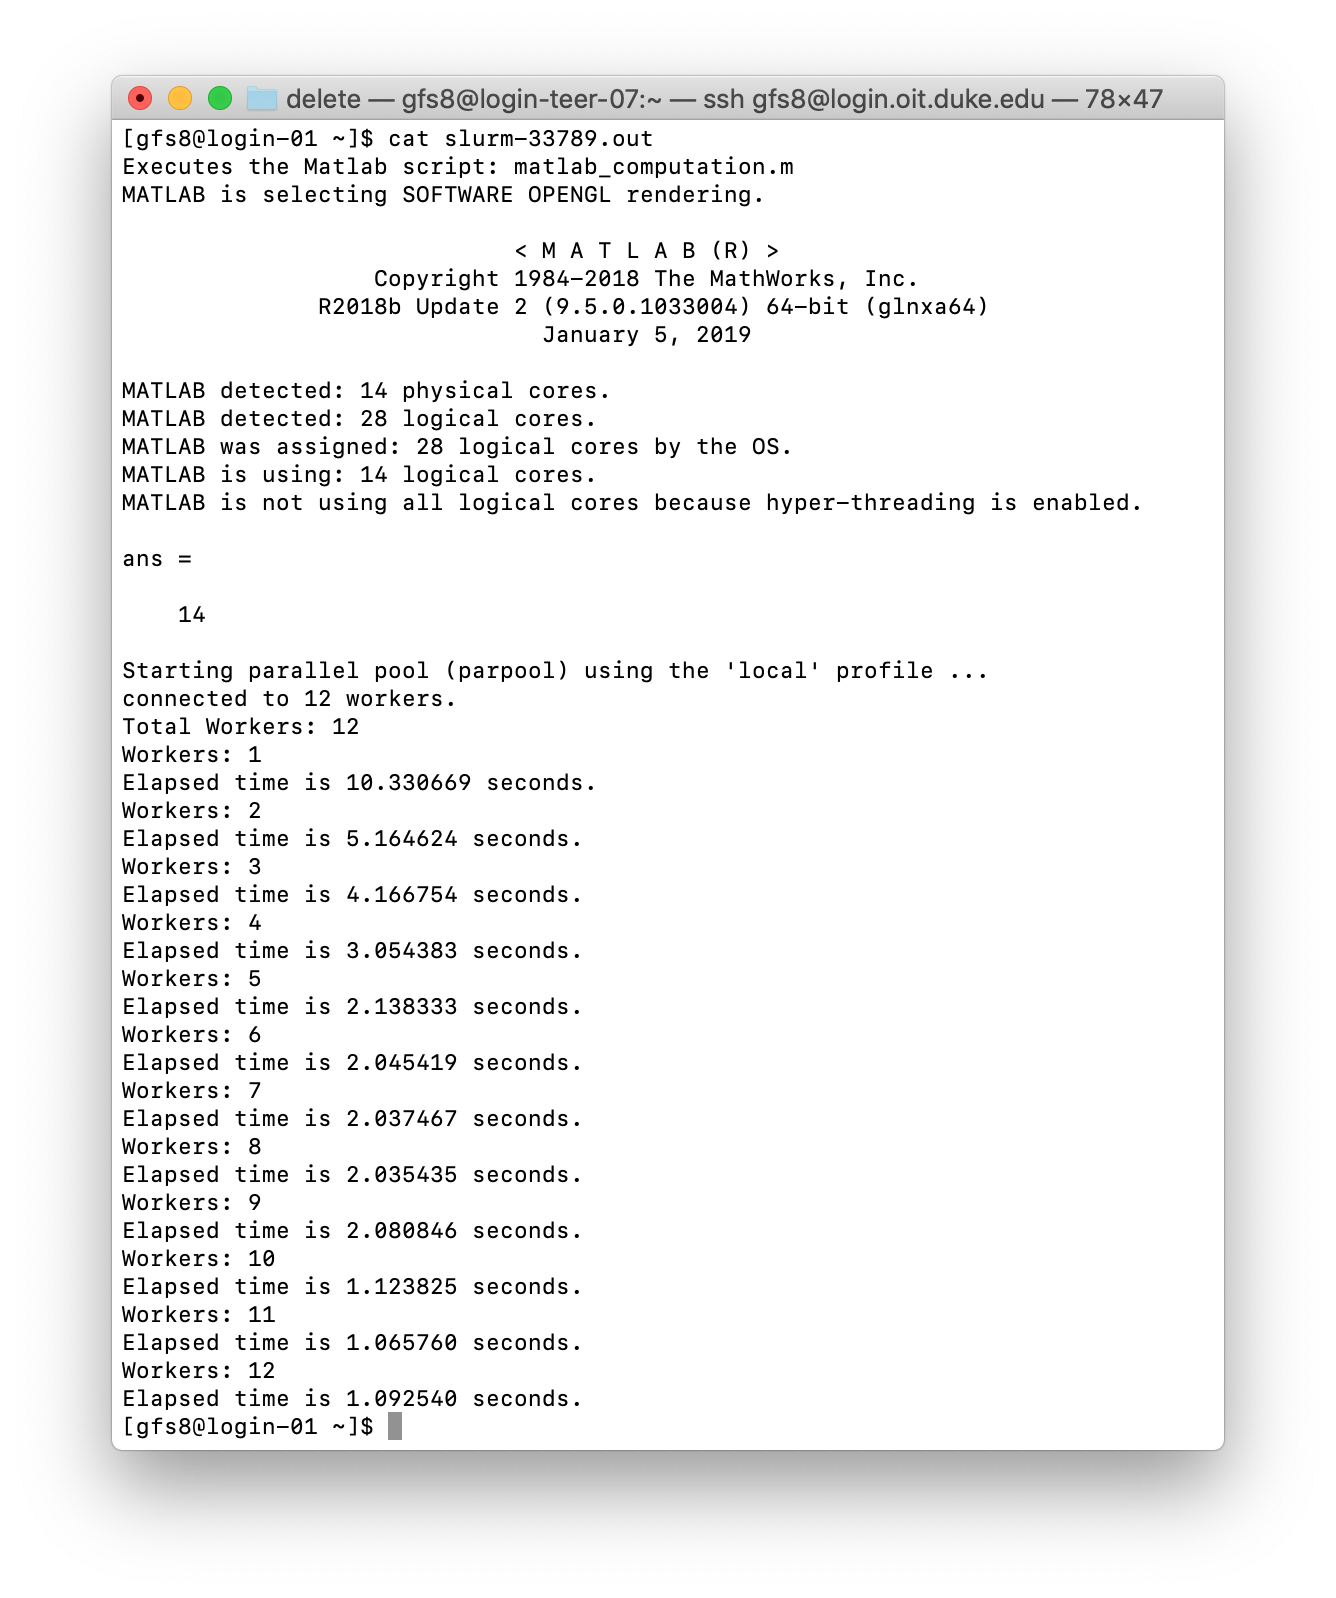
\includegraphics[width=8cm]{/Users/guilhermesalome/Teaching/Duke/Econ890 Matlab - 2019/supporting/matlab_cluster_parallel.png}
\caption{\label{fig:org4687b2a}
Output of Matlab script using \texttt{parfor} on the cluster.}
\end{figure}

In this case, even though we only requested four CPUS, many more were available.
Indeed, we could create a pool of workers with twelve workers!
Notice that there were actually fourteen cores available to Matlab, but the default number of workers from the \texttt{parpool} command is twelve.
We could have created a pool with the fourteen workers by calling \texttt{parpool(14)}.
Alternatively, we could have called \texttt{parpool(feature('numcores'))} to use all available cores.
\subsection{Multiple Jobs and Transferring Files}
\label{sec:org8527f2b}
We have discussed how to submit a single job that uses many cores to speed up computation.
An alternative paradigm is submitting several different jobs that use a single core, and then collecting all of their results.

For example, consider you have a statistic that you are interested in studying via bootstrap, but that takes a long time to be computed (potentially because of a large sample, or because the statistic is complicated).
In this case, we could launch several different jobs, where each computes a bootstrap sample and the statistic just once.
We can then accumulate the results to study the distribution of the statistic.

Let's create some fake data to bootstrap.
\lstset{language=matlab,label= ,caption= ,captionpos=b,firstnumber=1,numbers=left,style=Matlab-editor}
\begin{lstlisting}
% generate_fake_data.m
mu = 20.5;
sigma = 5.8;
sample_size = 1000000;
sample = normrnd(mu, sigma, sample_size, 1);
save('fake_data.mat', 'sample');
\end{lstlisting}
We will use this data to compute the confidence interval for the mean via bootstrap.
We need to get the data from our computer into the cluster.
To do so, we will use the command \texttt{scp}, which is similar to the \texttt{ssh} command, but is used to copy files securely.
If you are transferring a lot of files, or want a graphical user interface, then you could use the program \href{https://cyberduck.io}{Cyberduck}, for example.

The syntax for \texttt{scp} is the following:
\lstset{language=bash,label= ,caption= ,captionpos=b,firstnumber=1,numbers=left,style=bash}
\begin{lstlisting}
scp file_to_copy username@host:~
\end{lstlisting}
The command will take the file named \texttt{file\_to\_copy} and copy it to the folder \texttt{\textasciitilde{}} in the host.
Remember that \texttt{\textasciitilde{}} represents your home folder.

At the time of writing, I am outside of the Duke network, so there are two steps to copy the data from my laptop to the Econ Cluster.
First, I need to transfer the data from my laptop to the Duke login node.
Then, I \texttt{ssh} into the Duke login node and transfer the data from there to the Econ Cluster.
\lstset{language=bash,label= ,caption= ,captionpos=b,firstnumber=1,numbers=left,style=bash}
\begin{lstlisting}
# Locate the file on my laptop
ls -1
# fake_data.mat is in the current working directory
scp fake_data.mat gfs8@login.oit.duke.edu:~
# will ask for your password and then start transferring the file
# Now, ssh into the login node of Duke
ssh gfs8@login.oit.duke.edu
# check that fake_data.mat is in the current working directory
ls -1
# transfer to the Econ Cluster
scp fake_data.mat gfs8@login.econ.duke.edu:~
# ssh into the Econ Cluster
ssh gfs8@login.econ.duke.edu
# verify that the file was transferred
ls -1
\end{lstlisting}

Now, let's create the bootstrapping script.
\lstset{language=matlab,label= ,caption= ,captionpos=b,firstnumber=1,numbers=left,style=Matlab-editor}
\begin{lstlisting}
% bootstrap_mean_fake_data.m
% Load data
load('fake_data.mat', 'sample');
% Bootstrap a new sample
ssize = length(sample);
new_sample = sample(unidrnd(ssize, ssize, 1));
% Compute statistic
statistic = mean(new_sample);
% Save result to csv
% Question: but what should be the name of the file?
\end{lstlisting}
The script loads the fake data, generates a bootstrap sample, computes the statistic and saves it in a \texttt{.csv} file.
However, we have a problem. What should be the name of the \texttt{.csv} file?
Since we are launching multiple jobs at the same time, how do we set the name of the file programmatically?
Before answering these questions, let's create the \texttt{bash} script that will launch several jobs, where each job will execute the Matlab script above once.
\lstset{language=bash,label= ,caption= ,captionpos=b,firstnumber=1,numbers=left,style=bash}
\begin{lstlisting}
#!/bin/bash
# multiple_jobs.sh
#SBATCH --cpus-per-task=1
#SBATCH --mem=1GB
#SBATCH --array=1-10
matlab -batch "bootstrap_mean_fake_data"
\end{lstlisting}
We can use the \texttt{-{}-array} directive to submit multiple jobs with Slurm.
The directive \texttt{-{}-array=1-10} will launch ten different jobs, numbered from 1 to 10.
Each job will execute our Matlab script.
Since each job has a different number, each job will create a separate \texttt{.out} output file.
However, this output file is just what is displayed in the terminal, and is mainly used for debugging.
What we want to recover is the file containing the statistic we computed.

When we submit a job with \texttt{-{}-array}, a variable is created with the number of the number of the job.
We can pass this variable to the Matlab script and use it to save the statistic value.
The variable name that holds the job number is \texttt{SLURM\_ARRAY\_TASK\_ID}.
We can access its value in the \texttt{bash} script using the command \texttt{\$SLURM\_ARRAY\_TASK\_ID}.
We can then pass this value to the matlab script:
\lstset{language=bash,label= ,caption= ,captionpos=b,firstnumber=1,numbers=left,style=bash}
\begin{lstlisting}
#!/bin/bash
# multiple_jobs.sh
#SBATCH --cpus-per-task=1
#SBATCH --mem=1GB
#SBATCH --array=1-10
matlab -batch "job_number=$SLURM_ARRAY_TASK_ID; bootstrap_mean_fake_data"
\end{lstlisting}
Now, inside the \texttt{boostrap\_mean\_fake\_data.m} script we can access the variable \texttt{job\_number}:
\lstset{language=matlab,label= ,caption= ,captionpos=b,firstnumber=1,numbers=left,style=Matlab-editor}
\begin{lstlisting}
% bootstrap_mean_fake_data.m
% Set seed
rng(job_number);
% Load data
load('fake_data.mat', 'sample');
% Bootstrap a new sample
ssize = length(sample);
new_sample = sample(unidrnd(ssize, ssize, 1));
% Compute statistic
statistic = mean(new_sample);
% Save result to csv
filename = strcat(num2str(job_number), '.csv');
csvwrite(filename, statistic);
\end{lstlisting}
The variable \texttt{job\_number} is initialized by the \texttt{bash} script.
We use it to create the \texttt{.csv} file, so that each job, which has its own unique number, will create a unique \texttt{.csv} file.
This also has the advantage that if some job fails (a bug, or takes too much resource, or bad weather), then we can quickly find it.
We also used the \texttt{job\_number} to set the seed for random number generation.
This way when we generate the bootstrap samples they are not all going to be the same, and the output will be repeatable if executed with the same \texttt{job\_number}.

We can submit the script to Slurm and verify that indeed 10 jobs are created:
\lstset{language=bash,label= ,caption= ,captionpos=b,firstnumber=1,numbers=left,style=bash}
\begin{lstlisting}
# Submit script for execution
sbatch multiple_jobs.sh
# A job id is assigned.
# Look at all jobs that were created:
squeue -u gfs8
# Notice that JOBID is xxxxxx_y, where xxxxxx is the job id, and
# y is the job number specified in the --array directive
# Observe that many slurm-xxxxxx_y.out files were created:
ls -1 slurm-*
# The * above expands slurm- to all existing filenames that
# begin with slurm-
# Jobs should be done now:
squeue -u gfs8
# Notice that the .csv files were created
ls -1 *.csv
# We can sort the names numerically with the option -v
ls -1 -v *.csv
# We can print them on the screen with cat
cat *.csv
\end{lstlisting}

The directive \texttt{-{}-array} takes a range of numbers, like \texttt{1-10}, and launches jobs using those numbers to create the job ids.
However, the range of numbers can be discontinuous.
For example, the directive \texttt{-{}-array=1-3,5,7-10} would launch jobs with ids 1, 2, 3, 5, 7, 8, 9 and 10, skipping the ids 4 and 6.
It is also possible to use \texttt{-{}-array=7} to launch a single job with that id number.
The single value or discontinuous \texttt{-{}-array} directives are useful for resubmitting a specific job that failed.

\section{Assignment}
\label{sec:orgdc5b5cd}
\begin{problem}
Modify the scripts \texttt{multiple\_jobs.sh} and \texttt{bootstrap\_mean\_fake\_data.m} so that a new folder is created to store the resulting \texttt{.csv} files.
If the folder already exists, the files inside it should be deleted before the script runs.
\end{problem}

\begin{problem}
(Optional) Create a \texttt{bash} script that takes all of the \texttt{.csv} files outputted from \texttt{multiple\_jobs.sh} and creates a single \texttt{.csv} file with all of the results.
\end{problem}

\begin{problem}
Create a Matlab script that takes all of the \texttt{.csv} files outputted from \texttt{multiple\_jobs.sh} and creates a single \texttt{.csv} file with all of the results.
\end{problem}

\begin{problem}
Compare the advantages and disadvantages of the following takes on parallel computing with the cluster:
\begin{itemize}
\item Launching a single job that uses multiple cores;
\item Launching several jobs that use a single core.
\end{itemize}
\end{problem}

\begin{problem}
Assume you mistakenly launched several jobs with the \texttt{-{}-array=1-500000} directive. Instead of typing \texttt{scancel job\_id} for each job, how would you use \texttt{scancel} to cancel all of the jobs you submitted at once?
\end{problem}

\begin{problem}
Consider a deterministic growth model, where an agent decides between consumption (\(c_t\)) and investment in capital (\(k_t\)), while maximizing his utility.
We can write this problem as:
\begin{align*}
  \max&\sum_{t=0}^{\infty}\beta^tU(c_t)\\
  \text{subject to }&
                      \begin{cases}
                        k_{t+1} = k_t^{\alpha} - c_t + (1-\delta)k_t, \forall t >= 0\\
                        k_0 > 0
                      \end{cases}
\end{align*}
Write the problem as a \href{https://en.wikipedia.org/wiki/Bellman\_equation}{Bellman equation}.
Let \(U(c; \sigma)=\frac{c^{1-\sigma}-1}{1-\sigma}\).
Obtain the Euler equation for this problem in terms of the consumption \(c\).
Solve the problem by Value Function Iteration.
Consider \(\sigma=2\), \(\beta=0.95\), \(\delta=0.1\) and \(\alpha=0.33\).
Use the steady state value of \(k\) to create a grid for the possible values of \(k\), say \(100\) points between \(0.25 k^*\) and \(1.75 k^*\).
Start with a guess for \(V\) over the grid, for example \(V(k)=0\) for all \(k\) in the grid.
Use the Matlab minimization function to solve for \(k\).
You may want to add the constraint that \(c\) should always be positive.

Use \texttt{parfor} and the Econ Cluster to speed up the solution of this problem.
Compare the speed gain with solving the problem using your local computer.
\end{problem}

\newpage
\printbibliography
\newpage
\end{document}